% !TeX spellcheck = cs_CZ
{\tikzset{external/prefix={tikz/CES/}}
 \tikzset{external/figure name/.add={ch08_}{}}
%---------------------------------------------------------------------------------------------------
% file STM32.tex
%---------------------------------------------------------------------------------------------------
%==============================Kapitola: STM32 procesory============================================
%\setchaptertoc
\chapter{Mikroprocesory s architekturou ARM }
%\minitoc

\section{Historické mezníky vývoje ARM architektury}
  \textbf{\texttt{ARM}} je architektura procesorů vyvinutá v Británii firmou \texttt{ARM Limited}. 
  Starší obchodní název architektury \texttt{ARM} je \texttt{Advanced RISC Machine}, původní název 
  je \texttt{Acorn RISC Machine}. Tato architektura způsobila v několika směrech revoluci v 
  informačních technologiích. Její návrh se řídil filosofií \texttt{RISC}, neméně pozoruhodné je, 
  že první procesory \texttt{ARM} byly založeny na \texttt{GaAs} polovodičích, které dovolily na 
  tehdejší dobu velmi vysoké taktovací frekvence. Rovněž použitá 32bitová šířka slova nebyla v době 
  vzniku \texttt{ARMu} samozřejmostí. První mikroprocesor s architekturou ARM byl navržen firmou 
  ARM Limited v roce 1984.
  
  Firma \texttt{ARM Limited} časem ustoupila od výroby procesorů a místo toho se soustředila pouze 
  na jejich vývoj. Schéma procesorů \texttt{ARM} je tedy \emph{"intelektuálním vlastnictvím"} firmy 
  \texttt{ARM}, která od výrobců hardware vybírá licence za jeho použití. Procesory \texttt{ARM} je 
  dnes možné najít ve všech odvětvích spotřební elektroniky od PDA, mobilních telefonů, 
  multimediálních přehrávačů, přenosných herních konzolí, kalkulaček až po počítačové periferie 
  (pevné disky, routery). Procesory \texttt{ARM} mají ve svém výrobním programu desítky výrobců 
  (ST, NXP, TI, Atmel,..).
  
  Architektura ARM se nejvýrazněji uplatňuje ve vestavěných systémech. Nízká spotřeba energie při 
  vysokém výpočetním výkonu má zásadní význam hlavně v zařízeních napájených bateriemi, avšak je 
  velkou výhodou také u zařízení pracujících v náročných tepelných podmínkách.
  
  \begin{figure}[ht!]
    \centering
    \begin{tabular}{c}
      \subfloat[Architektura v7A]{\label{MIT:fig_CortexM3}
        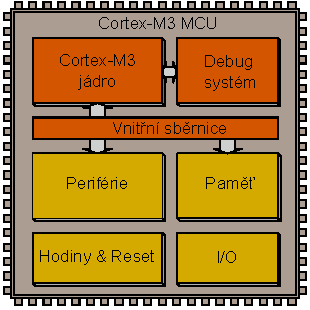
\includegraphics[width=0.3\textwidth]{CortexM3_block.pdf}}              \\
       \begin{tikzpicture}
         \node[below left] at (0,-1) {aa};
       a \newline
       a       
       \end{tikzpicture}
       \begin{tikzpicture}
    %  \node[below left] at (0,0) {Legenda: }; 
    %   \tikzset{every node/.style={rectangle split, draw, minimum width=.2cm}}
    %   \node[rectangle split part fill={red!50}] {a};
     \draw (0,0) rectangle (0.5,0.5);
     \fill[green!20!white] (0,0) -- (3mm,0mm) arc (0:30:3mm) -- cycle;
       \end{tikzpicture} 
            \\
    \end{tabular}
    \caption{Příklady architektur rodiny Cortex ARM}
  \end{figure}
  
\section{Architektura ARMv7}
  Tato architektura je rozdělená do tří úrovní - profilů.
  \begin{itemize}\addtolength{\itemsep}{-0.5\baselineskip}
    \item Profil A (ARMv7-A; série Cortex-A) je určen pro komplexní aplikace a operační systémy  
          jako je například Linux nebo Windows Embedded, které potřebují výkonný procesor, podporu 
          virtuální paměti jednotkou správy paměti (MMU) a případně hardwarovou podporu aplikací 
          napsaných v programovacím jazyku Java.
    \item Profil R (ARMv7-R; série Cortex-R) je určen především pro real-time systémy, které 
          potřebují vysoký výpočetní výkon a krátkou dobu reakce.
    \item Profil M (ARMv7-M; série Cortex-M) je určen pro mikrokontroléry, kde je potřebný  
          dostatečný výkon procesoru, rychlá odezva na přerušení, ale hlavním kritériem je nízká 
          cena a spotřeba energie.
  \end{itemize}
  
  \begin{figure}[ht!]
    \centering
    \begin{tabular}{c}
      \subfloat[Architektura v7A]{\label{MIT:fig_CortexA8_basicArch}
        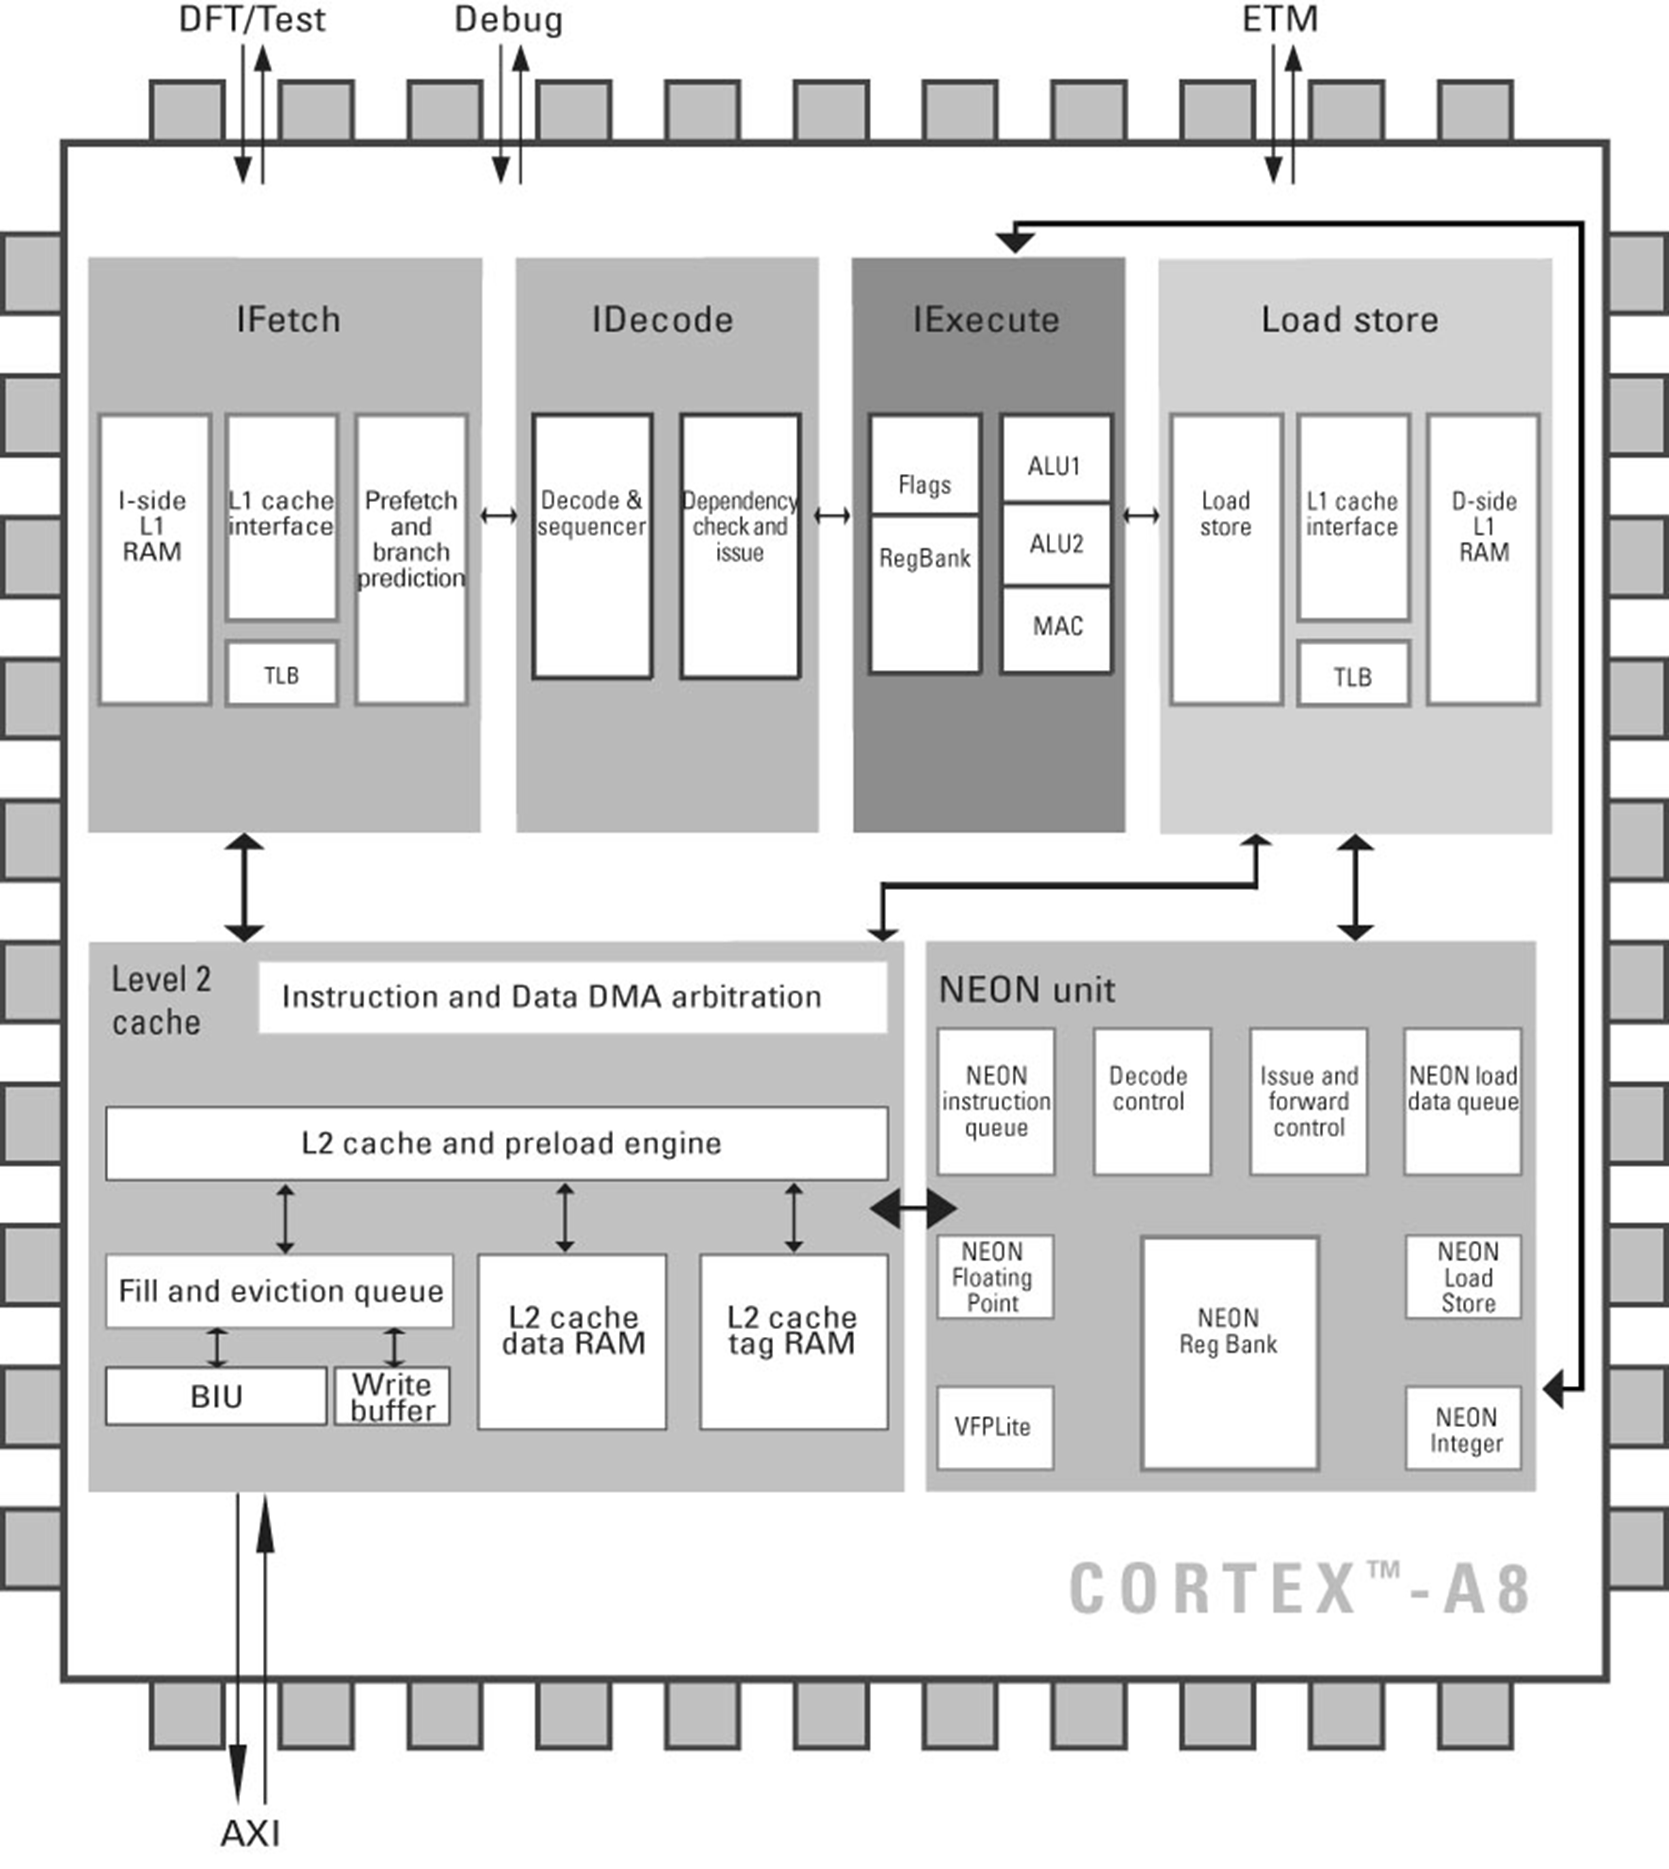
\includegraphics[width=0.3\textwidth]{CortexA8_basicarch.png}}              \\
      \subfloat[Architektura v7R]{\label{MIT:fig_CortexR4_basicArch} 
        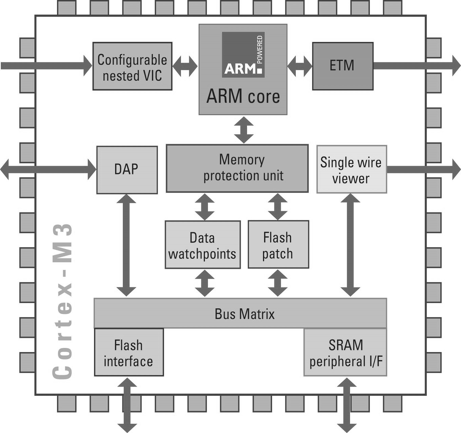
\includegraphics[width=0.3\textwidth]{CortexM3_basicarch.png}}              \\
      \subfloat[Architecture v7M]{\label{MIT:fig_CortexM3_basicArch} 
        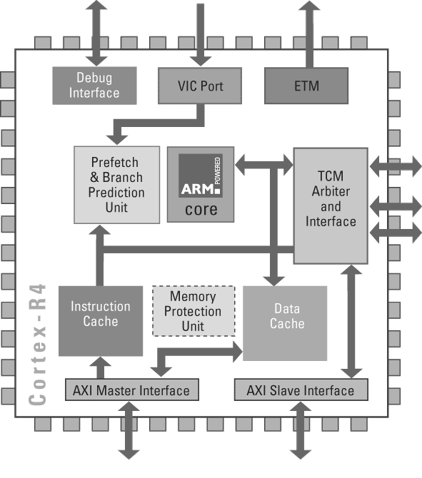
\includegraphics[width=0.3\textwidth]{CortexR4_basicarch.png}}
    \end{tabular}
    \caption{Příklady architektur rodiny Cortex ARM}
  \end{figure}

 
\section{Architektura mikroprocesoru STM32F100xx}
  Jádro Cortex-M3 je založeno na Harvardské architektuře (kap. \ref{MIT:chap_adr_prostor}), která 
  má oddělenou sběrnici pro data a pro instrukce. To umožňuje rychlejší vykonávání programového 
  kódu, kdy je možné paralelně načítat novou instrukci a zároveň ukládat data výsledku do paměti. 
  Toho se využívá při pipeliningu (zřetězování instrukcí nebo průtokové zpracování instrukcí[5]), 
  který má 3 fáze - načtení instrukce, dekódování instrukce a vykonání instrukce. Zároveň se také 
  odhaduje, zda může aktuálně vykonávaná instrukce větvení ovlivnit aktuálně načítanou a 
  dekódovanou instrukci. Mechanismus pipeliningu tím umožňuje mnohonásobné zvětšení výkonu vzhledem 
  k hodinovému kmitočtu jádra mikrokontroléru.  
  \begin{figure}[ht!] %\ref{MIT:fig_stm32f100arch}
    \centering
    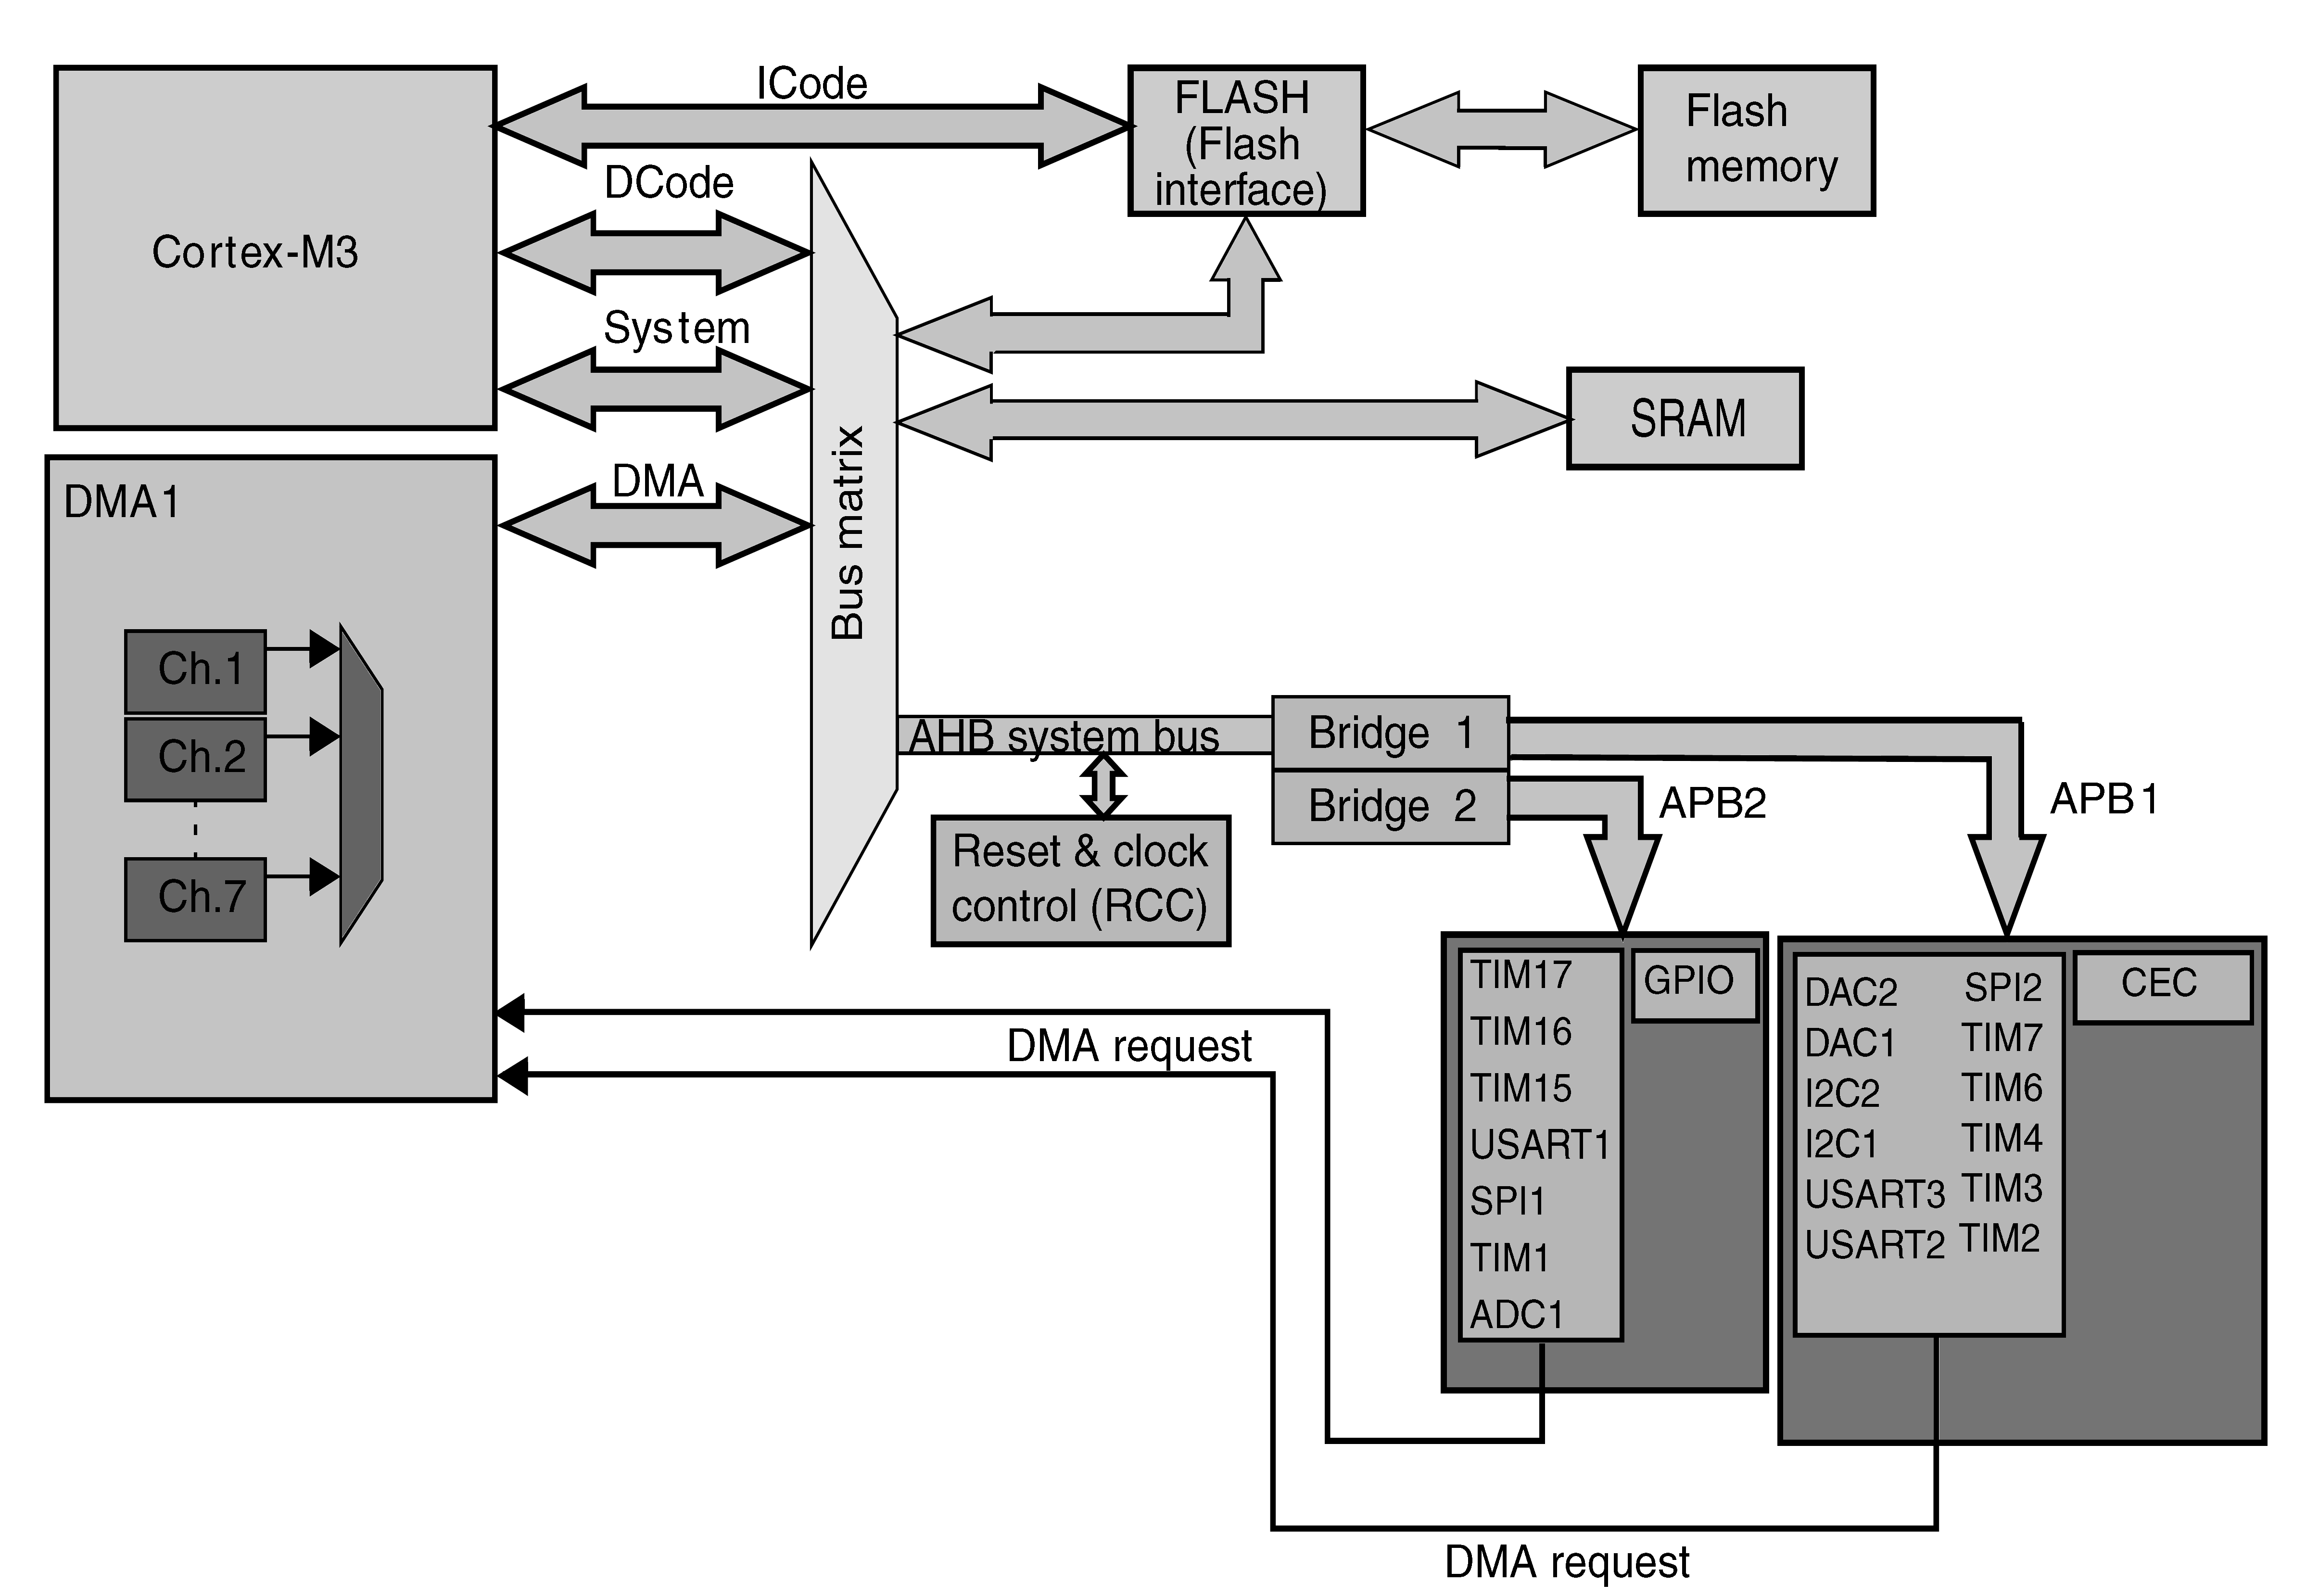
\includegraphics[width=1\linewidth]{STM32F100_arch.png}
    \caption{Architektura systému nízké a střední hustoty řady Value Line}
    \label{MIT:fig_stm32f100arch}
  \end{figure}
  
  \subsection{Reset and clock control (RCC)}
  
\section{CMSIS}
  \begin{itemize}
    \item \href{http://librarian/stable.php?id=141}{CMSIS Tutorial}
  \end{itemize}
  
} % tikzset
%---------------------------------------------------------------------------------------------------
%\printbibliography[title={Seznam literatury}, heading=subbibliography]
\addcontentsline{toc}{section}{Seznam literatury}